\chapter {Kako locirati mutacije koje izazivaju bolesti?}
\setbookcodestyle

\section{Mapiranje očitavanja}

Cena sekvencionisanja genoma je od 2001. u konstantnom padu, i teži se tome da ono postane potpuno pristupačno običnom čoveku, kao i da bude sastavni deo lekarske usluge.

\iffalse
\begin{figure}[h!]
\centering
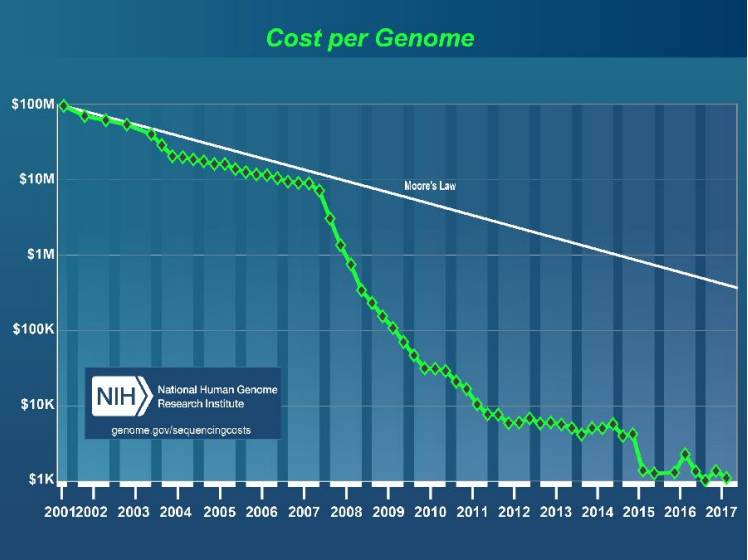
\includegraphics[scale=0.7]{poglavlja/9/slike/CostPerGenom.png}
\caption{Kretanje cene sekvencioniranja u poslednjih 17 godina}
\label{slika:X}
\end{figure}
\fi 

Oko 1\% dece rodi se sa mentalnom retardacijom, ali uzroci ove pojave i dan-danas nisu razjašnjeni, jer do nje može dovesti niz različitih genetskih poremećaja. Jedan od njih je i Ohdo sindrom, koji izaziva bezličan ,‚maskoliki'' izraz lica. 
Biolozi su 2011. godine uspeli da pronađu niz zajedničkih mutacija kod pacijenata, koje su kasnije iskorišćene za identifikovanje jedintvene mutacije proteina, odgovorne za nastanak ovog sindroma. Razumevanje suštinskog uzroka Ohdo sindroma samo je jedno od otkrića do kojeg se došlo proučavanjem genetskih poremećaja upotrebom \textbf{mapiranja očitavanja}. 
Kod ove metode, porede se sekvencionisana očitavanja DNK uzeta od pojedinaca sa \textit{referentnim ljudskim genomom}. 

\textbf{Referentni ljudski genomom} zamišljen je da bude ‚‚prosečan'' ljudski genom izračunat na određenom broju uzoraka. Trenutni referentni genom baziran je na genomima 13 dobrovoljaca iz SAD-a; i dalje se vrši njegovo usavršavanje ispravljanjem grešaka i popunjavanjem rupa (trenutno ih je preko stotinu). U proseku, razlika između individualnog i referentnog genoma je u oko 3 miliona mutacija.

\iffalse 
\begin{figure}[h!]
\centering
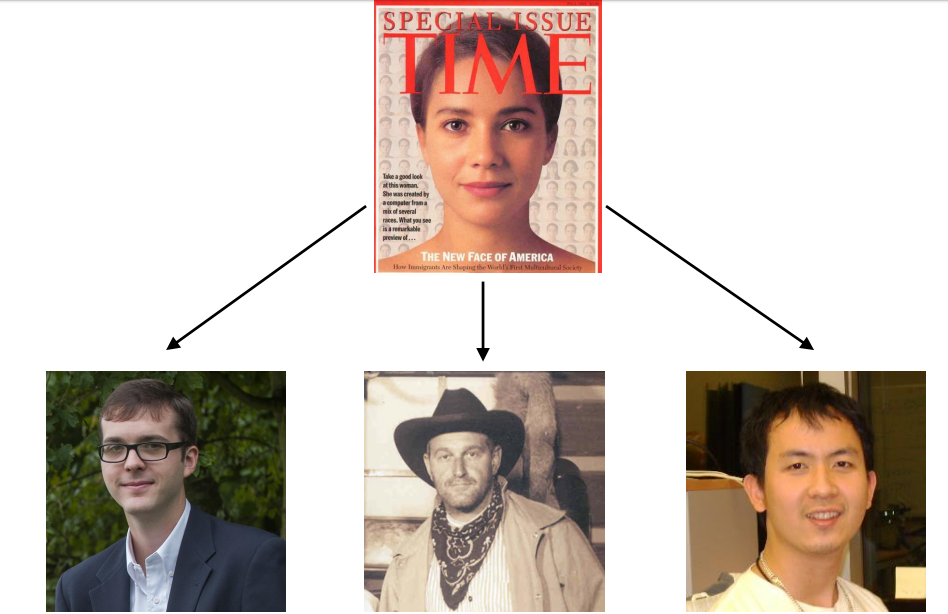
\includegraphics[scale=0.5]{poglavlja/9/slike/OdGenomaVrsteDoPersonalnih.png}
\caption{Prikaz grananja genoma vrste na više personalnih genoma}
\label{slika:X}
\end{figure}


\begin{figure}[h!]
\centering
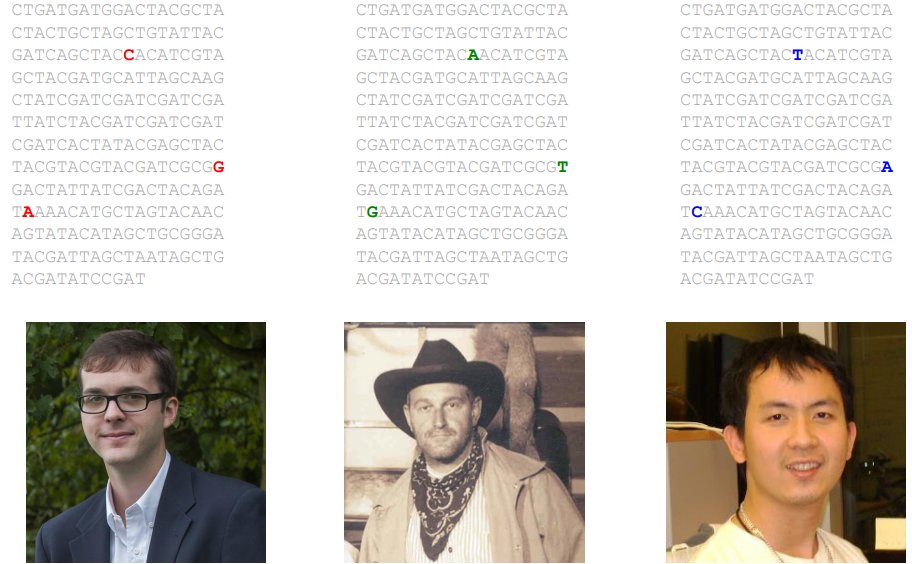
\includegraphics[scale=0.5]{poglavlja/9/slike/OdGenomaVrsteDoPersonalnih2.png}
\caption{Razlike u personalnim genomima}
\label{slika:X}
\end{figure}

\fi 

Pitanje je kako možemo efikasno sastaviti individualne genome koristeći referentne. Možemo koristiti \textbf{asembliranje}, ali konstrukcija de Brojnovog grafa zahteva mnogo memorije. Možemo koristiti postojeću strukturu referentnog genoma kao pomoć u sekvencioniranju genoma pacijenta.

\iffalse 
\begin{figure}[h!]
\centering
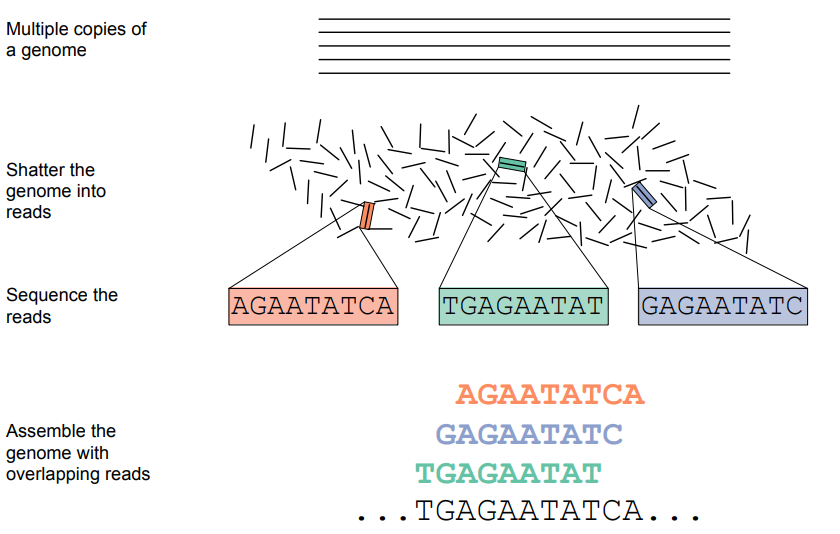
\includegraphics[scale=0.5]{poglavlja/9/slike/asembliranje.png}
\caption{Primer asembliranja}
\label{slika:X}
\end{figure}
\fi

\textbf{Mapiranje očitavanja} predstavlja određivanje pozicije u referentnom genomu sa kojima svako očitavanje ima visoku sličnost. Podsetimo se da su očitavanja izlaz sekvencera, dakle, neki sitni delovi genoma. 

\begin{figure}[h!]
\centering
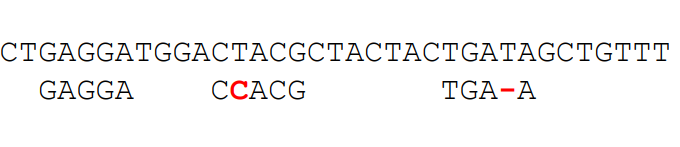
\includegraphics[scale=0.5]{poglavlja/9/slike/mapiranjeOcitavanja.png}
\caption{Primer mapiranja očitavanja; gornja niska predstavlja referentni genom, a donje niske očitavanja individualnog genoma}
\label{slika:X}
\end{figure}

\subsection{Egzaktno uparivanje šablona}
Potrebno je pronaći gde se očitavanja egzaktno poklapaju sa referentnim genomom. Postoji jednostruko i višestruko uparivanje šablona. Egzaktno u smislu da nema insercija i delecija.

\begin{tcolorbox}
\textbf{Problem jednostrukog uparivanja šablona:} \\
\indent \textbf{Ulaz:} Niske \textit{Pattern} i \textit{Genome}. \\
\indent \textbf{Izlaz:} Sve pozicije u niski \textit{Genome} gde se niska \textit{Pattern} pojavljuje kao podniska.
\end{tcolorbox}

\begin{tcolorbox}
\textbf{Problem višestrukog uparivanja šablona:} \\
\indent \textbf{Ulaz:} Kolekcija niski \textit{Patterns} i \textit{Genome}. \\
\indent \textbf{Izlaz:} Sve pozicije u niski \textit{Genome} gde se niske iz kolekcije \textit{Patterns} pojavljuju kao podniske.
\end{tcolorbox}


\subsection{Rešenje grubom silom}

Rešenje koje nam prvo pada na pamet je rešavanje problema grubom silom. Algoritam se sastoji u tome da se linearno krećemo kroz genom i proveravamo da li se dati šablon poklapa sa podniskom genoma iste dužine, koja počinje na toj poziciji.


\begin{minipage}{\textwidth}
	\centering
	\begin{minipage}{0.45\textwidth}
		\begin{figure}[H]
			\centering
			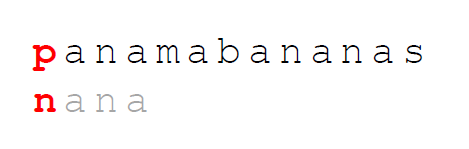
\includegraphics[width=\textwidth]{poglavlja//9/slike/GrubaSilaGreska.png}
			\caption{Uparivanje šablona grubom silom - nepoklapanje}
			\label{bfNepoklapanje}
		\end{figure} 
	\end{minipage}
	\hfill 
	\begin{minipage}{0.45\textwidth}
		\begin{figure}[H]
			\centering
			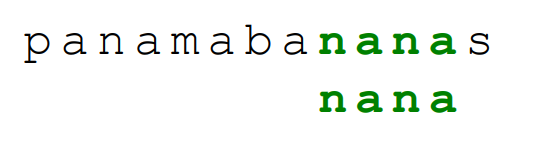
\includegraphics[width=\textwidth]{poglavlja/9/slike/GrubaSilaPogodak.png}
			\caption{Uparivanje šablona grubom silom - poklapanje}
			\label{bfPoklapanje}
		\end{figure}  
	\end{minipage}
	\vspace*{1em}
\end{minipage}

Vreme izvršavanja algoritma u slučaju jednostrukog \textit{Pattern}-a je $O(|Genome| * |Pattern|)$, dok je u slučaju višestrukog \textit{Patterns}-a je $O(|Genome| * |Patterns|)$, gde je \textit{|Patterns|} suma dužina elemenata liste \textit{Patterns}. 

Međutim, problem je u tome što genomi mogu biti veoma dugi. U slučaju ljudskog genoma (3 GB), ukupna dužina svih očitavanja može biti veća od 1 TB; kao rezultat toga, algoritam složenosti $O(|Genome| * |Patterns|)$ je previše spor.

U nastavku smo u potrazi za efikasnijim algoritmom, ali i pogodnijom strukturom podataka. U algoritmu svakom koraku radimo poređenje iznova, što dovodi do neefikasnosti. 

\subsection{Sufiksna stabla}
Razlog velike neefikasnosti prethodnog algoritma jeste u tome što paterni prolaze kroz genom nezavisno jedan od drugog. Ako nisku \textit{Genome} zamislimo kao put, onda bi izvršavanje algoritma grube sile bilo analogno vožnji svakog paterna po putu u zasebnom automobilu. Ono što želimo jeste da sve paterne smestimo u jedan ‚‚autobus'', čime bi nam bio dovoljan samo jedan prolazak kroz nisku \textit{Genome}. Zbog toga paterne organizujemo u strukturu podataka nalik na usmereni aciklički graf, koju nazivamo \textbf{Trie} i koja ima sledeće osobine:

\begin{itemize}
    \item Trie ima jedinstven čvor sa ulaznim stepenom nula, koji nazivamo koren
    \item Svaka grana Tria je obeležena jednim slovom
    \item Grane koje izlaze iz jednog čvora obeležene su različitim slovima
    \item Svaki sufiks neke niske dobija se nadovezivanjem slova duž neke putanje grafa, idući od korena naniže
    \item Svaka putanja stabla od korena do lista, ili do čvora sa izlaznim stepenom 0, predstavlja jedan element iz liste \textit{Patterns}
\end{itemize}

Najjednostavniji način konstrukcije strukture Trie jeste iterativno dodavanje niski iz niza \textit{Patterns} u rastuću strukturu. Za date niske Text i Trie(Patterns) možemo brzo proveriti da li se neki element niza Patterns predstavlja prefiks niske Text. Dovoljno je da krenemo da spelujemo Text i da slovo po slovo prolazimo kroz Trie od korena naniže. Za svako slovo iz Text-a gledamo da li iz trenutnog čvora postoji grana obeležena tim slovom; ukoliko postoji, nastavljamo sa pretragom; u suprotnom obustavljamo pretragu i zaključujemo da nijedan element niza Patterns nije prefiks niske Text. Ukoliko stignemo do lista, onda je pretraga bila uspešna.

Da bismo pronašli da li se neki patern nalazi u genomu, potrebno je da u $\|Text\|$ iteracija pokrećemo prethodno opisani algoritam, pri čemu u svakoj iteraciji iz niske Text izbacujemo početni simbol, sve dok ona ne postane prazna.

Iako je prethodno opisani postupak vremenski efikasan, njegova mana leži u velikom zauzeću memorije. Naime, veličina strukture Trie proporcionalna je  ukupnom broju simbola niza Patterns, a pošto veličina kolekcije očitavanja ljudskog genoma može dostići 1 TB, memorija potrebna za čuvanje ove strukture je prevelika.


Bolji pristup je da se struktura Trie pravi na osnovu niske Text, tj. genoma. Za ovo će nam biti struktura poznata kao \textbf{sufiksni trie}. \textbf{Sufiksni trie} date niske predstavlja trie formiran na osnovu svih sufiksa te niske. Pre konstrukcije sufiksnog stabla, na kraj niske dodajemo simbol \$, kako bismo kasnije znali kad smo stigli do kraja.

Proveru da li se dati patern nalazi u tekstu vršimo tako što tražimo put u sufiksnom stablu, spelujući slova paterna do kraja. Ukoliko dođe do nepoklapanja, pretraga je neuspešna. U suprotnom, pretraga je uspešna. Primer jednog nekompresovanog sufiksnog stabla nalazi se na slici \ref{nss}.


\begin{minipage}{\textwidth}
	\centering
	\begin{minipage}{0.45\textwidth}
		\begin{figure}[H]
			\centering
			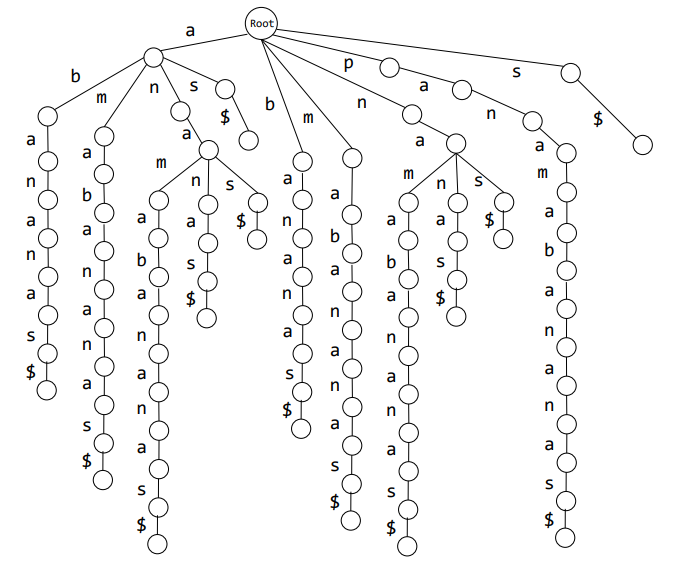
\includegraphics[width=\textwidth]{poglavlja/9/slike/sufiksnoStabloNekompresovano.png}
			\caption{Nekompresovano sufiksno stablo}
			\label{nss}
		\end{figure} 
	\end{minipage}
	\hfill 
	\begin{minipage}{0.5\textwidth}
		\begin{figure}[H]
			\centering
			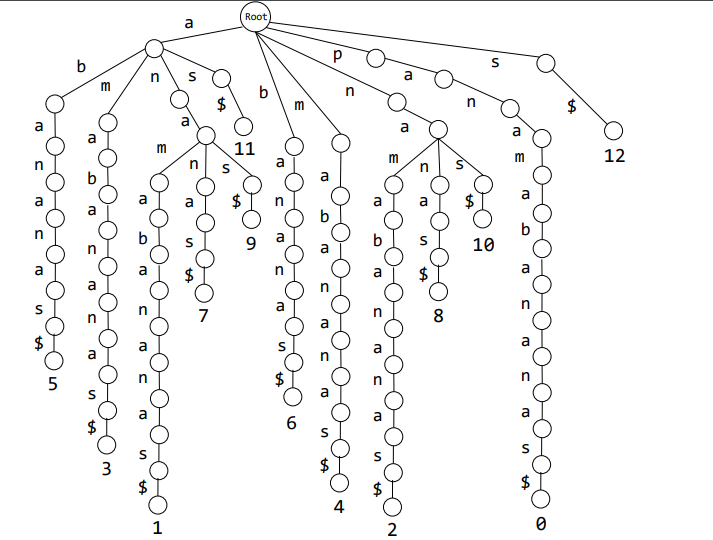
\includegraphics[width=\textwidth]{poglavlja/9/slike/sufiksnoStabloNumerisaniPrefiksi.png}
			\caption{Sufiksno stablo sa numerisanim prefiksima}
			\label{nssNum}
		\end{figure}  
	\end{minipage}
	\vspace*{1em}
\end{minipage}

\iffalse 
\begin{figure}[h!]
\centering
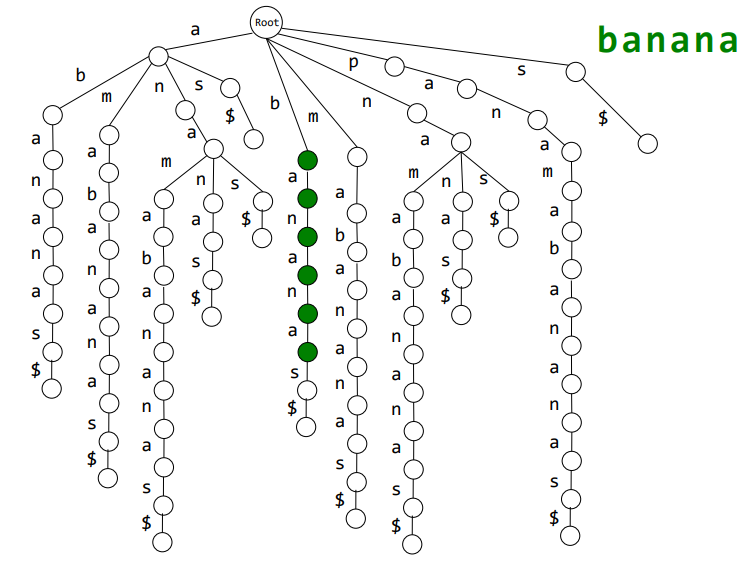
\includegraphics[scale=0.5]{poglavlja/9/slike/sufiksnoStabloNekompresovanoPogodak.png}
\caption{Nekompresovano sufiksno stablo - uspešno pronalaženje niske}
\label{slika:X}
\end{figure}

\begin{figure}[h!]
\centering
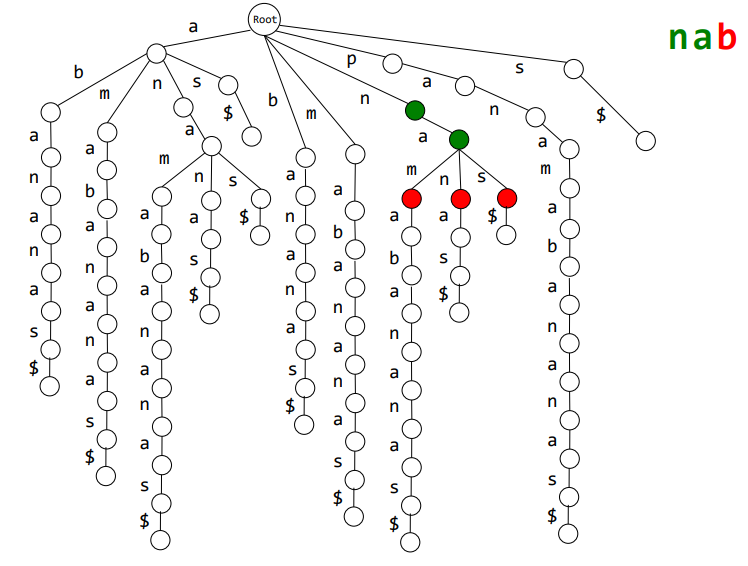
\includegraphics[scale=0.5]{poglavlja/9/slike/sufiksnoStabloNekompresovanoGreska.png}
\caption{Nekompresovano sufiksno stablo - neuspešno pronalaženje niske}
\label{slika:X}
\end{figure}
\fi 

Ovim postupkom možemo utvrditi da li se pattern pojavljuje u genomu, ali ne i na kojoj poziciji. Za to moramo dodati još informacija u stablo. Na svakom listu dodamo početnu poziciju u niski Genome sufiksa koji se završava u tom listu, kao na slici \ref{nssNum}.


Sad se postavlja pitanje, kada pronađemo uparivanje, kako da znamo na kojoj poziciji se ono nalazi. To je sada lako, kada pronađemo uparivanje, nastavimo sa kretanjem naniže do lista, gde se nalazi pozicija odakle počinje pojavljivanje podniske. 

\iffalse 
\begin{figure}[h!]
\centering
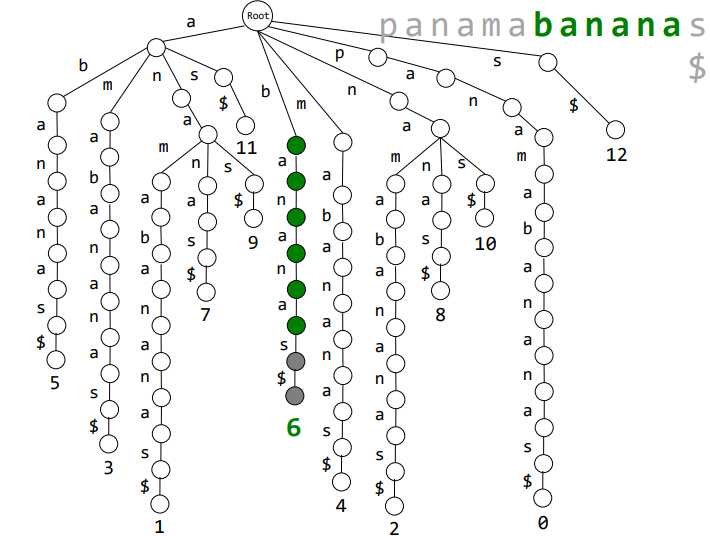
\includegraphics[scale=0.5]{poglavlja/9/slike/sufiksnoStabloNaciIndeksPocetka.png}
\caption{Primer nalaženja pozicije nakon uparivanja}
\label{slika:X}
\end{figure}

\begin{figure}[h!]
\centering
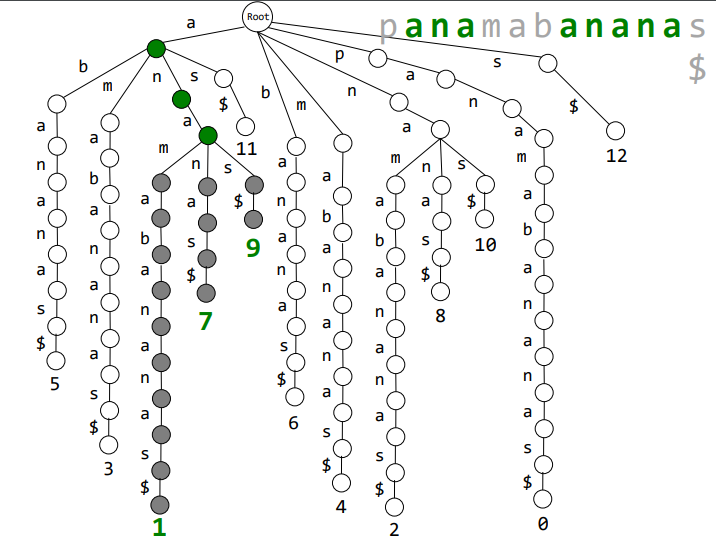
\includegraphics[scale=0.5]{poglavlja/9/slike/sufiksnoStabloNaciIndeksPocetkaVise.png}
\caption{Primer nalaženja pozicije nakon uparivanja - više poklapanja}
\end{figure}
\fi 


Da bismo smanjili prostornu složenost, možemo kompresovati svaku putanju koja se ne grana u jednu granu. Ovakva struktura podataka naziva se \textbf{sufiksno stablo}. Kompresovano sufiksno stablo prikazano je na slici \ref{kss}.

Za svaku nisku \textit{Genome} važi da je ukupan broj čvorova manji od dvostruke dužine niske \textit{Genome}, tj. $\# nodes < 2|Genome|$. Ovo važi na osnovu činjenice da je broj listova jednak dužini genoma, tj. $\# leaves = |Genome|$, odnosno da je broj unutrašnjih čvorova manji od dužine genoma umanjene za jedan, tj. $\# internal nodes < |Genome| - 1$.

\begin{figure}[h!]
\centering
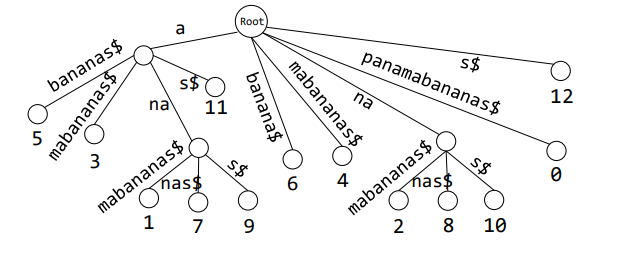
\includegraphics[scale=0.5]{poglavlja/9/slike/sufiksnoStabloKompresovano.png}
\caption{Kompresovano sufiksno stablo}
\label{kss}
\end{figure}

\noindent\textbf{Vremenska složenost} za konstrukciju sufiksnog stabla tako što se prvo konstruiše nekompresovano sufiksno stablo je O($|Genome|^2$), a za nalaženje uparivanja O($|Patterns|$). \textbf{Prostorna složenost}  za konstrukciju sufiksnog stabla tako što se prvo konstruiše nekompresovano sufiksno stablo je O($|Genome|^2$), a  za čuvanje sufiksnog stabla O($|Patterns|$).

Postoje algoritmi sa linearnom prostornom i vremenskom složenošću. Vremenska složenostza konstrukciju sufiksnog stabla direktno  O($|Genome|$), a za nalaženje uparivanja je O($|Patterns|$) što ukupno iznosi O($|Genome|$ + $|Patterns|$). Prostorna složenost za konstrukciju sufiksnog stabla direktno O($|Genome|^2$), a za čuvanje sufiksnog stablaO($|Patterns|$) što ukupno iznosi O($|Genome|$).

\section{Kompresija niski i Barouz-Vilerova transformacija}

Najveći problem koji se javlja sa prethodnom rešenjem je to što O-notacija ignoriše konstante, a najpoznatija implementacija sufiksnih stabala zahteva ~ 20 * |Genome| (npr. veličina humanog genoma je 3GB => 60 GB; i dalje unapređenje u odnosu na 1TB). Postavlja se pitanje da li možemo smanjiti faktor konstante. Odgovor nam daje kompresija genoma.

\subsection{Kompresija genoma}

Glavna ideja ovog rešenja jeste da se smanji količina memorije potrebna za čuvanje niske Genome. Za ovo su nam potrebne metode za kompresiju niske velikih dužina, što je naizgled sasvim drugačiji problem.

U ovom genomu imamo nekoliko uzastopnih ponavljanja jedne aminokiseline (ranovi, runs): prvo uzastopna ponavljanja aminokiseline G, pa C i tako dalje), a u nekim imamo uzastopna ponavljanja nizova aminokiselina (ripitsi, repeats): prvo uzastopna ponavljanja GAC, pa CATT i tako dalje.

\begin{figure}[H]
	\centering
	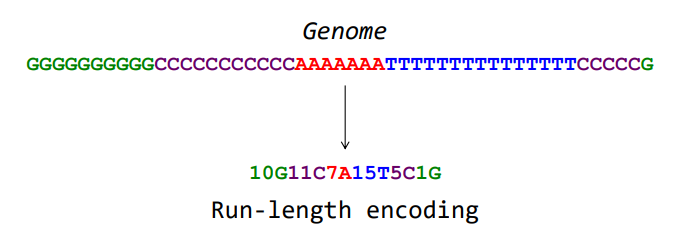
\includegraphics[scale=0.5]{poglavlja/9/slike/kompresijaGenoma.png}
	\caption{}
	\label{slika:X}
\end{figure}

Prva ideja pri rešavanju ovog problema jeste da kodiramo dužine ranova. Problem kod ovog pristupa jeste to što u genomu nema mnogo ranova. Međutim, ima mnogo ripita. Postavlja se pitanje kako izvesti transformaciju ripita u ranove.  Znamo kako da kodiramo dužinu ranova. Imamo genomsku sekvencu \textit{Genome} i ona sigurno sadrži neke ripite. Međutim, za njih ne znamo kodiranje. Možemo konvertovati nisku u \textit{Genome*} koja predstavlja nisku u kojoj su se ripiti konvertovali u ranove. A, kada to uradimo, onda znamo kako da kodiramo ranove i dobijamo \textit{CompressedGenome}. 

Kako onda kodiramo ripite u ranove? Odgovor na ovo pitanje daje nam Barouz-Vilerova transformacija (The Burrows-Wheeler Transform, skraćeno BWT).
 


\iffalse 
\begin{figure}[h!]
\centering
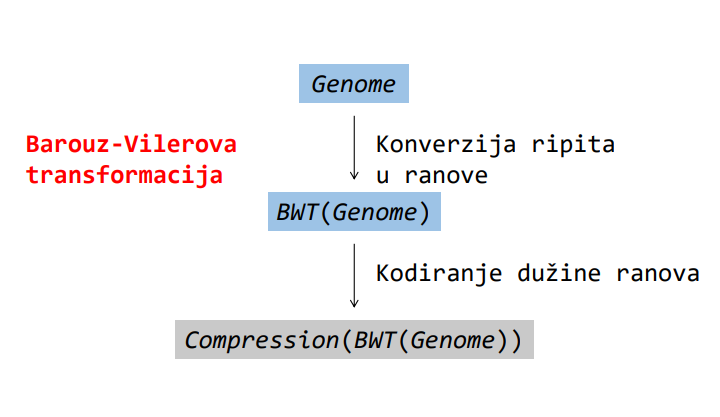
\includegraphics[scale=0.5]{poglavlja/9/slike/konversijaRipitaUranove.png}
\caption{}
\label{slika:X}
\end{figure}
 
\begin{figure}[h!]
\centering
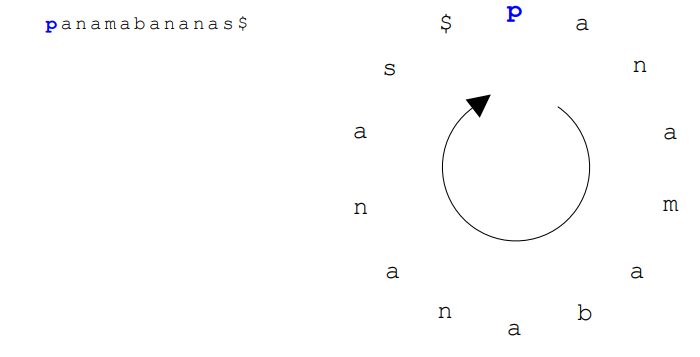
\includegraphics[scale=0.6]{poglavlja/9/slike/BWT.png}
\caption{}
\label{slika:X}
\end{figure}
\fi

Ideja kod ovog algoritma je da se na početku formiraju sve ciklične rotacije date niske.

\begin{figure}[h!]
\centering
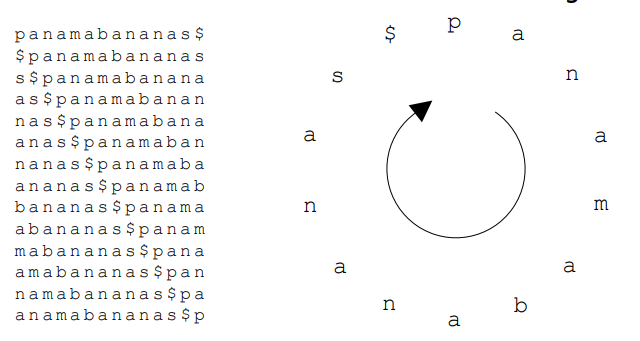
\includegraphics[scale=0.7]{poglavlja/9/slike/SveCiklicneRotacije.png}
\caption{Scenario sa 4 promene}
\label{slika:X}
\end{figure}

Takvu kolekciju niski sortiramo leksikografski (\$ je na početku).
\iffalse 
\begin{figure}[h!]
\centering
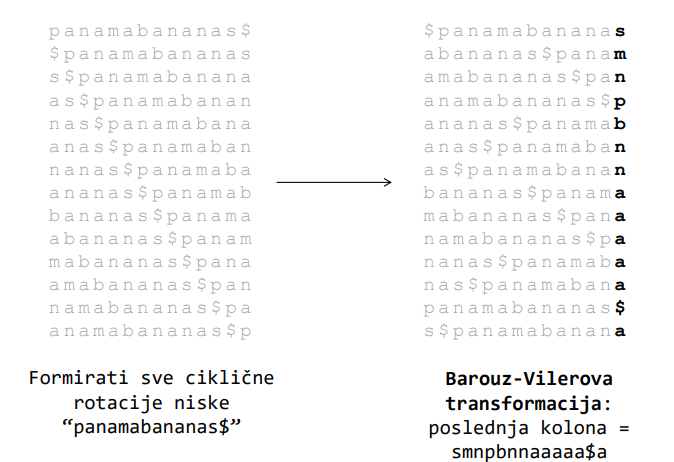
\includegraphics[scale=0.4]{poglavlja/9/slike/BWTPoslednjaKolona.png}
\caption{}
\label{slika:X}
\end{figure}
\fi 
BWT je u ovako sortiranoj kolekciji niski poslednja kolona. Možemo primetiti da poslednja kolona sadrži veliki broj ranova. Međutim, isti slučaj je i sa prvom kolonom. Prvo ćemo se pozabaviti dekompresijom dobijene niska, pa ćemo se posle vratiti na ovo pitanje.


\section{Inverzna BWT}


\iffalse 
\begin{figure}[h!]
\centering
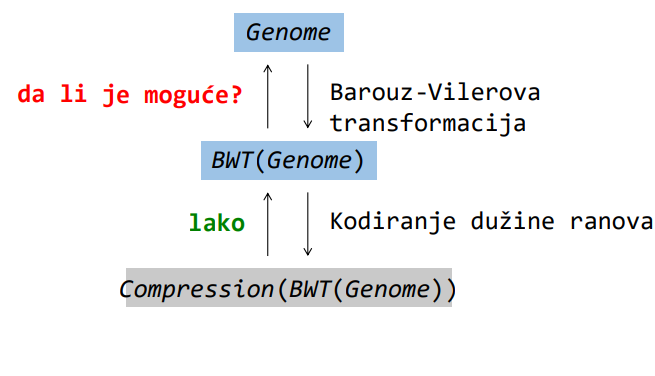
\includegraphics[scale=0.5]{poglavlja/9/slike/KakoDekompresiju.png}
\caption{}
\label{slika:X}
\end{figure}
\fi 

Pogledajmo primer BWT-a za nisku ‚‚\textit{banana}''. Ako sortiramo karaktere poslednje kolone ‚‚annb\$aa'', dobićemo prvu kolonu matrice. Na osnovu toga znamo 2-gramski sastav cirkularne niske \textit{banana\$}. Sortiranjem niski dobijamo prve dve kolone matrice. Sada imamo dve kolone cikličnih niski. Zatim ponavljamo postupak - dodamo poslednju koju znamo, itd. Na kraju dobijamo rekonstruisanu celu matricu


\iffalse 
\begin{figure}[h!]
\centering
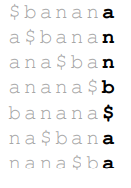
\includegraphics[scale=0.5]{poglavlja/9/slike/banana.png}
\caption{}
\label{slika:X}
\end{figure}

\begin{figure}[h]
\centering
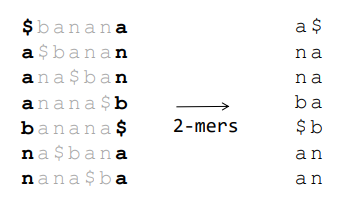
\includegraphics[scale=0.7]{poglavlja/9/slike/2-gramskiSastav.png}
\caption{}
\label{slika:X}
\end{figure}
\fi 


\begin{figure}[h!]
\centering
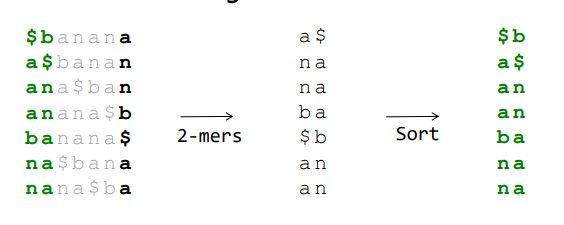
\includegraphics[scale=0.5]{poglavlja/9/slike/2-gramskiSastav2.png}
\caption{}
\label{slika:X}
\end{figure}

Nisku banana\$ dobijamo tako što uzmemo sve elemente iz prvog reda posle \$.
\textbf{Prostorna složenost:} Rekonstrukcija niske Genome na osnovu BWT(Genome) zahteva čuvanje |Genome| kopija niske Genome, što iznosi O($|Genome|^2$). Poboljšanje složenosti je moguće ako primetimo neobično svojstvo.

\textbf{First-Last} svojstvo: k-to pojavljivanje simbola u FirstColumn i k-to pojavljivanje simbola u LastColumn odgovaraju istoj poziciji simbola u niski Genome.

Ako na slici \ref{firstLast} posmatramo prvi karakter 'a' u prvoj koloni, i prvi karakter 'a' u poslednjoj koloni, primetićemo da se te dve niske razlikuju samo za to 'a', odnosno razlikuju se po tome što je karakter 'a' kod prve niske u prvoj koloni, a kod druge u poslednjoj koloni. To važi i za ostale niske.

Hajde da proverimo da li ovo uvek važi. Posmatramo prvu kolonu i vidimo da se karakter 'a' pojavljuje u 6 cikličnih rotacija na prvom mestu. Izdvojimo te niske i prvu kolonu (tj. karakter 'a') i dobijamo kolekciju koja je i dalje sortirana. Zatim dodamo karakter 'a' na kraj, i dalje imamo sortirane niske. I to su niske koje se nalaze u ostatku kolekcije, gde je 'a' na kraju.   

\begin{figure}[h!]
\centering
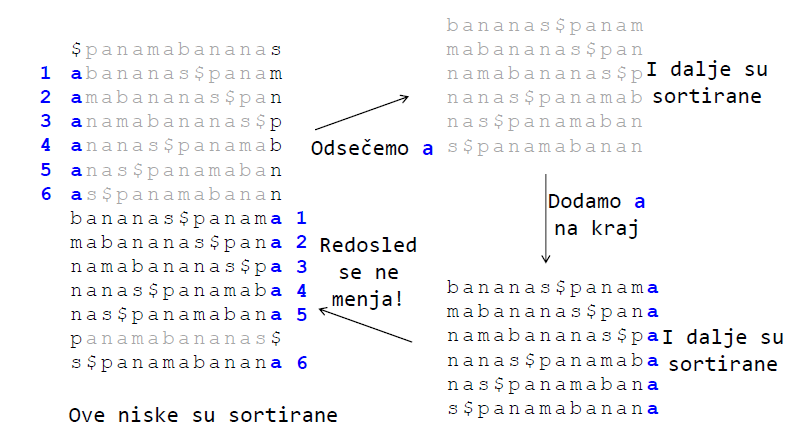
\includegraphics[scale=0.6]{poglavlja/9/slike/firstLast.png}
\caption{First-Last svojstvo}
\label{firstLast}
\end{figure}

\subsection{Efikasnija BWT dekompresija}

Krenemo od simbola \$ (prvi u nizu cikličnih niski) u FirstColumn, zatim pogledamo koji simbol je u LastColumn u tom redu, nađemo ga u FirstColumn, onda za taj red nađemo koji simbol je u tom redu u LastColumn, itd. U jednom trenutku ćemo doći do \$ u LastColumn i tada smo okrenuli ceo krug i rekonstruisali celu Genome nisku. Prostorna složenost je 2|Genome| = O(|Genome|).


\subsection{Korišćenje BWT za uparivanje šablona}

Da se podsetimo, uparivanje šablona korišćenjem sufiksnih stabala zahtevalo je vremensku složenost od O(|Genome| + |Patterns|), prostorna O(|Genome|). Problem je bio što je sufiksno stablo tražilo 20 * |Genome| prostora. Poboljšanje možemo dobiti ako umesto sufiksnog stabla koristimo BWT(Genome) kao strukturu podataka.

Postupak se sastoji od toga da krenemo od kraja niske koju tražimo i u FirstColumn nađemo taj karakter. Zatim u odgovarajućem redu u LastColumn tražimo drugi od pozadi karakter od tih kojima je u FirstColumn poslednji iz uzorka.

Zatim nađemo u FirstColumn gde su ti iz LastColumn i gledamo naredni karakter. Ako se poklapa sa trećim od pozadi, nastavljamo dalje, ako ne, nema ga. I tako dok ne pređemo ceo uzorak od kraja ka početku.

Pogledajmo to na primeru. Tražimo nisku ‚‚ana'' u niski ‚‚panamabananas\$''. U prvoj koloni imamo 6 niski koje počinju karakterom 'a'. Posmatramo poslednju kolonu i tražimo slovo 'n'. Takvih kolona ima tri, ostale nećemo dalje razmatrati. Karakteri 'a' kojima prethodni 'n' obeleženi su redom brojevima 2, 5 i 6. Tražimo tri niske koje počinju karakterom 'n' (obeleženi su sa n1, n2 i n3). Gledamo šta se nalazi iza karaktera 'n', to su sve karakteri 'a' (oni obeleženi brojevima 2, 5 i 6), što je očekivano jer su to oni karakteri 'a' koje smo malo pre pronašli u prvoj koloni. Zatim, posmatramo poslednju kolonu i odbacujemo niske koje nam ne odgovaraju. Kako se sve tri niske završavaju karakterom 'a', nećemo nijednu isključiti. Ovi karakteri 'a' obeleženi su brojevima 3, 4, 5. Prelazimo u redove gde se nalaze a3, a4 i a5 i pronalazimo da sve tri sadrže nisku ‚‚ana''. 

Kao što vidimo, možemo da koristimo BWT reprezentaciju za uparivanje šablona. Međutim, nismo dobili odgovor na pitanje na kojim pozicijama se nalaze ova pojavljivanja. Možemo dobiti odgovor da li se nalazi i koliko puta se pojavljuje.


\begin{minipage}{\textwidth}
	\centering
	\begin{minipage}{0.45\textwidth}
		\begin{figure}[H]
			\centering
			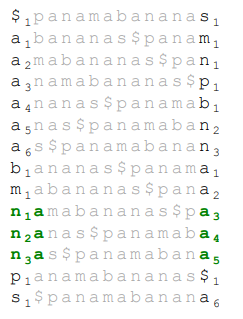
\includegraphics[width=\textwidth]{poglavlja/9/slike/traziAnukraj1.png}
			\caption{First-Last svojstvo}
			\label{ana1}
		\end{figure} 
	\end{minipage}
	\hfill 
	\begin{minipage}{0.45\textwidth}
		\begin{figure}[H]
			\centering
			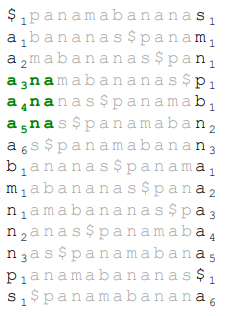
\includegraphics[width=\textwidth]{poglavlja/9/slike/traziAnukraj2.png}
			\caption{First-Last svojstvo}
			\label{ana2}
		\end{figure}  
	\end{minipage}
	\vspace*{1em}
\end{minipage}


\subsection{Pronalaženje uparenih šablona}

\begin{tcolorbox}
\textbf{Problem višestrukog uparivanja šablona:}\\
\textbf{Ulaz:} Kolekcija niski Patterns i niska Genome.\\
\textbf{Izlaz:} Sve pozicije u niski Genome gde se niske iz kolekcije Patterns pojavljuju kao podniske.
\end{tcolorbox}

Treba da nađemo pozicije. BWT ne daje ovaj podatak. Na primer, na gornjem primeru ‚‚ana'' se pojavljuje 3 puta, ali na kojim pozicijama? To ćemo odrediti pomoću sufiksnog niza.

\textbf{Sufiksni niz} je niz koji čuva početnu poziciju za svaki sufiks (niz karaktera u svakom redu matrice do simbola \$) i prikazan je na slici \ref{sufiksniNiz}.


\begin{figure}[h!]
\centering
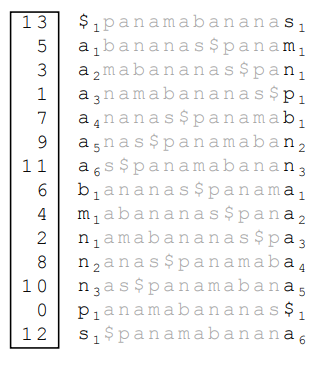
\includegraphics[scale=0.75]{poglavlja/9/slike/sufiksniNiz.png}
\caption{Sufiksni niz}
\label{sufiksniNiz}
\end{figure}

Sa slike vidimo da se ‚‚ana'' iz prethodnog primera pojavljuje na pozicijama 1, 7 i 9.

Da li smo pokvarili složenost? Prostorna složenost je $4 * |Genome|$ (ako koristimo 4B za cele brojeve kao elemente niza), što je bolje nego $20 * |Genome|$. Sufiksni niz jeste poboljšanje, ali nije najbolje poboljšanje. Postoji prisup sa $|Genome|$ prostornom složenosti, a koristi  parcijalni sufiksni niz. Ovim se nećemo dalje baviti.

\section{Približno preklapanje}

Do sad smo definisali problem egzaktnog poklapanja i način na koji ga možemo rešiti. Ponekad je neophodno pronaći približna uparivanja šablona. Približno znači da se neće sve pozicije poklapati. Baš te pozicije predstavljaju mutacije do kojih je došlo zbog čega nam je približno poklapanje značajno. 

\begin{tcolorbox}
	\textbf{Približno uparivanje šablona:}\\
	\textbf{Ulaz:} Niska Pattern, niska Genome, ceo broj d (kod višestrukog uparivanja ulaz je kolekcija niski Patterns).\\
	\textbf{Izlaz:} Sve pozicije niske Genome, gde se niska Pattern pojavljuje kao podniska sa najviše d razlika.
\end{tcolorbox}

Analogno egzaktnom uparivanju, postoji i problem višestrukog približnog uparivanja šablona koji opisujemo u nastavku. 


\begin{tcolorbox}
	\textbf{Višestruko približno uparivanje šablona:} \\
	\textbf{Ulaz:} Kolekcija niski Pattern, niska Genome, ceo broj d (kod višestrukog uparivanja ulaz je kolekcija niski Patterns). \\
	\textbf{Izlaz:} Sve pozicije niske Genome, gde se niska Pattern pojavljuje kao podniska sa najviše d razlika.
\end{tcolorbox}


Hajde da vidimo na primeru kako možemo primeniti BWT na približno preklapanje.  Pretpostavimo da je $d=1$. Traženje preklapanja radimo kao i pre, samo što sada prihvatamo i kad imamo različite karaktere. Zbog toga, sada zadržavamo i crvena slova, kao na slici \ref{anaMiss1}, sve dok je broj razlika $\leq d$. Čuvaćemo informaciju o broju nepoklapanja i svuda gde smo odabrali crveno slovo broj nepoklapanja se uvećava za jedan. 

Sada tražimo niske koje počinju karakterima koje smo odabrali u prethodnom koraku (m1, n1, p1, b1, n2, n3), odnosno tražimo ih u prvoj koloni. Naravno, te vrste se završavaju sa a. Treba da utvrdimo šta se nalazi ispred, odnosno na kraju, u poslednjoj koloni. Sve niske, osim one koja počinje sa p1, završavaju se sa 'a', što nam ne povećava broj nepoklapanja. Niska koja počinje sa p1 završava sa '\$', što uvećava broj nepoklapanja na 2. Tu nisku ćemo odbaciti jer je premašen broj nepoklapanja. 

Tako smo pronašli pet 3-grama koji imaju najviše 1 nepoklapanje, a na osnovu sufiksnog niza možemo videti gde su početne pozicije tih 3-grama.


\begin{minipage}{\textwidth}
	\centering
	\begin{minipage}{0.45\textwidth}
		\begin{figure}[H]
			\centering
			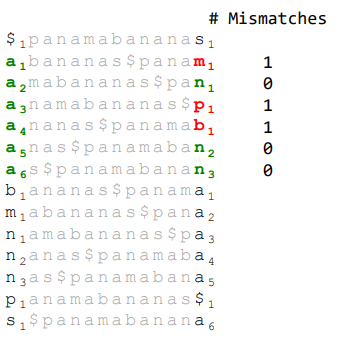
\includegraphics[width=\textwidth]{poglavlja/9/slike/PribliznoPreklapanjeMissmatch.png}
			\caption{Traženje približnog preklapanja za d = 1}
			\label{anaMiss1}
		\end{figure} 
	\end{minipage}
	\hfill 
	\begin{minipage}{0.45\textwidth}
		\begin{figure}[H]
			\centering
			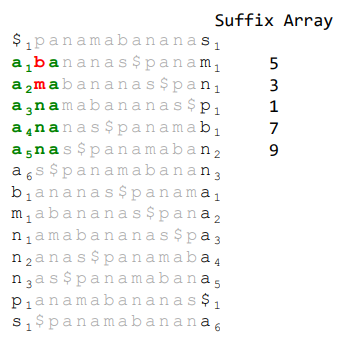
\includegraphics[width=\textwidth]{poglavlja/9/slike/PribliznoPreklapanjeTrazenjeNiske.png}
			\caption{Pozicije u genomu gde se javljaju približna preklapanja}
			\label{anaMiss2}
		\end{figure}  
	\end{minipage}
	\vspace*{1em}
\end{minipage}


\iffalse 
\section{Zadaci sa vezbi}

\setexamplecodestyle
\subsection{TrieConstruction}
\lstinputlisting[language=Python]{poglavlja/9/kodovi/TrieConstruction.py}

\subsection{SuffixArray}
\lstinputlisting[language=Python]{poglavlja/9/kodovi/SuffixArray.py}

\subsection{SuffixArrayMultiple}
\lstinputlisting[language=Python]{poglavlja/9/kodovi/SuffixArrayMultiple.py}

\subsection{BWT}
\lstinputlisting[language=Python]{poglavlja/9/kodovi/BWT.py}
\fi 